%\documentclass[a4paper,10pt]{article}
\documentclass[10pt]{article}
\usepackage[utf8]{inputenc}
\usepackage{xspace}
\usepackage{url}
\usepackage{graphicx,graphics} 
\usepackage{color}
\usepackage{amsmath}
\usepackage{amsfonts}
\usepackage{amssymb}
\usepackage{amsthm}
\usepackage{algorithm}
\usepackage{algorithmic}
\usepackage{longtable}
\usepackage{complexity}
\usepackage{tkz-graph}
\usepackage{float}
\usepackage{tabularx}
\usepackage{setspace}
\usepackage{icomma}
\renewcommand{\algorithmicrequire}{\textbf{Input:}}
\renewcommand{\algorithmicensure}{\textbf{Output:}}
\usepackage{authblk}
\usepackage[colorlinks=true,breaklinks=true,linkcolor=blue]{hyperref}


\newcommand\rmatching{${\cal R}$-matching\xspace}
\newcommand\mdelay{$\cal M$-delay\xspace}
\newcommand\matchedgraph{{\bf matched graph}}
\newtheorem{proposition}{Proposition}
\newtheorem{theorem}{Theorem}
\DeclareMathOperator{\pdv}{pdv}
\setlength{\parskip}{1ex} % Espace entre les paragraphes

\newtheorem{fact}{Fact}
\newtheorem{lemma}[theorem]{Lemma}
\newtheorem{definition}{Definition}
\newtheorem{corollary}{Corollary}

% \renewcommand{\thefootnote}{\*}

\newcommand{\todo}[1]{{\color{red} TODO: {#1}}}
\newcommand\pazl{\textsc{pazl}\xspace}
\newcommand\pall{\textsc{pall}\xspace}
\newcommand\bra{\textsc{bra}\xspace}
\newcommand\pra{\textsc{pra}\xspace}
\newcommand\minpra{\textsc{min-pra}\xspace}
%opening
\title{Deterministic Scheduling of Periodic Messages for Cloud RAN}
 

\author[1]{Dominique Barth}
\author[1,2]{Ma\"el Guiraud}
% \author[1]{Christian Cad\'er\'e}
 \author[2]{Brice Leclerc}
 \author[2]{Olivier Marc\'e}
\author[1]{Yann Strozecki}
\affil[1]{David Laboratory, UVSQ}
\affil[2]{Nokia Bell Labs France}

\begin{document}
We define by {\bf delay} of a datagram $d$ in a node $u_i$ of a route $r$, the time taken by the datagram to go from $u_0$, the first vertex of the route to $u_i$ through $r$. It is then equal to $DL(d,u_i,r) = t(d,u_j,r) - t(d,u_0,r)$. 
 Thus, the delay of a datagram in the node $u_i$ is equal to $DL(d,u_i,r) =  t(d,u_i,r) - t(d,u_0,r) = \lambda(u_i,r) + \sum_{k=0}^{i-1}( b(d,u_k,r) + l(d,u_k,r))$.
This delay is composed of three factors:
\begin{enumerate}
\item $\lambda(u_i,r)$ : it is the {\bf physical delay} of the route. This time is not alterable. 
\item  $\sum_{k=0}^{i-1} b(d,u_k,r)$ : those values correspond to some {\bf physical buffers } induced by the potential speedup or slowdown of the different links of the route used.
\item $\sum_{k=0}^{i-1} l(d,u_k,r)$: are the {\bf logical buffers}, chosen by the solution proposed to solve the problem. Those buffers are chosen by some algorithmic solutions in order to control the traffic in every node, and thus avoid collisions.
\end{enumerate}

As a reminder, a stream is a sequence of datagram. Each period, the sequence of datagrams $\{d_0,\ldots,d_{k-1}\}$, is sent on a route. The sequence of datagram is the same in every period: the same number of datagram which are of the same size are sent at the same tic in the period. For instance if the sequence $\{d_0,\ldots,d_{k-1}\}$ is sent at the first period P on the route r at times $\{\theta_r(d_0),\ldots,\theta_r(d_{k-1})\}$ then the datagrams $\{d_k,\ldots,d_{2k-1}\}$ will be send in the second period at times $\{\theta_r(d_k),\ldots,\theta_r(d_{2k-1})\}$, with $\theta_r(d_i) = \theta_r(d_i+k) \mod P, \forall i \in [0,\ldots,k-1]$. We say that two datagrams $d_i$ and $d_{i+k}$ are associated. The size in tics of two associated datagrams is always the same

\todo{Parler du fait que ce model peut a la fois couvrir un mode paquet et un mode circuit, indifféremment }


The {\bf packet delay variation ($\pdv$) }\cite{demichelis_ip_nodate} is the variation of the delay between two datagram. In our study, we allow some datagrams to be buffered in some nodes of the route, thus, the $\pdv$ between $d_0$ and $d_i$ (with $i<k$) can be greater than $0$. Formally, we denote the packet delay variation between two datagrams $d_i$ and $d_j$ in a node $u$ on a route $r$ by $\pdv(d_i,d_j,u,r) = |DL(d_i,u,r) - DL(d_j,u,r) | \ge 0$. 
\todo{dire que cette définition viens du monde ip mais que pour nous elle est considérée sur des datagrams ethernet}

Note that the $\pdv$ between two associated datagrams is always equal to zero, since the logical delays are deterministic, computed on a period and then applied to all the next periods.

\begin{center}
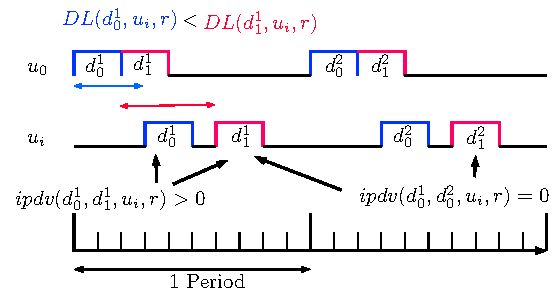
\includegraphics[width=0.8\textwidth]{ipdv}
  \end{center}
  
Let us introduce the notion of {\bf jitter} \cite{guillemin_peak_1992} , which is commonly used in statistical networks to define the variance of the packet delay variations in a node. In the case of a deterministic network, $\pdv$ is only due to the logical buffers, which also are deterministic. 

Thus, we can define the jitter in a deterministic point of view:
\begin{itemize}
\item The jitter of a datagram, is exactly equal to the sum of all the logical buffers applied to this packet (3.).
\item The jitter of a stream, is the maximum of the jitters of the datagram composing the steam.
\end{itemize}

One can observe that there is a bijection between our notion of jitter and $\pdv$, thus, to avoid confusion, we will not talk about jitter but the $\pdv$. 


\todo{quelques lignes sur la perte de paquets, dire qu'elle serait éventuellement acceptable}
\bibliographystyle{ieeetr}
\bibliography{srcs}

\end{document}
